\section{问题三：相关性与可替代/互补性下的最优种植策略（基于 Copula 的情景）}
为刻画“\textbf{销量—价格—成本}”之间的\textbf{相关性}以及作物间的\textbf{替代性/互补性}，问题三在问题二的情景优化框架上进一步引入：\emph{（i）高斯 Copula 生成的相关随机情景}；\emph{（ii）交叉价格弹性 $\varepsilon_{ij}$ 对需求的修正}；\emph{（iii）同样的 CVaR 风险约束与 GA 求解}。实现见 \verb|problem3.py|（文件名 \texttt{p3\_ga\_copula.py}），其核心流程为：构建 $3C\times 3C$ 的相关矩阵 $\Sigma$（$C$ 为作物数，对应 \{需求D、价格P、成本C\} 三块），用最近正定（nearest-PD）处理后进行 Copula 采样；再按预设的 $\varepsilon_{ij}$ 将需求对价格相对变动进行线性响应修正；最后以“期望利润 $-\ \lambda \cdot \mathrm{CVaR}_{95\%}(\text{亏损})$”为适应度，用遗传算法搜索 2024--2030 年、两季、全地块的作物配置，并将结果写回模板。:contentReference[oaicite:0]{index=0}

\subsection{相关结构设定与验证}
\paragraph{相关矩阵与 Copula 构造} 设作物索引为 $i=1,\dots,C$，将每个作物的 $(D_i, P_i, C_i)$ 串接形成向量 $X\in\mathbb{R}^{3C}$，并手工给出块结构相关矩阵 $\Sigma$：同作物内部 $D\text{--}P$ 为负相关（需求对价格的反向响应），$P\text{--}C$ 为正相关（价格与成本的共振）；跨作物之间，价格块按“同类作物相关更高”的原则设置，成本块较高相关，$D\text{--}P$ 交叉块由 $\varepsilon_{ij}$（替代 $>0$、互补 $<0$）诱导。经最近正定化后，对应得到高斯 Copula 的相关结构；以对数正态边际将 $u=\Phi(Z)$ 反变换到 $(D,P,C)$ 的连续分布。:contentReference[oaicite:1]{index=1}

\begin{figure}[htbp]
  \centering
  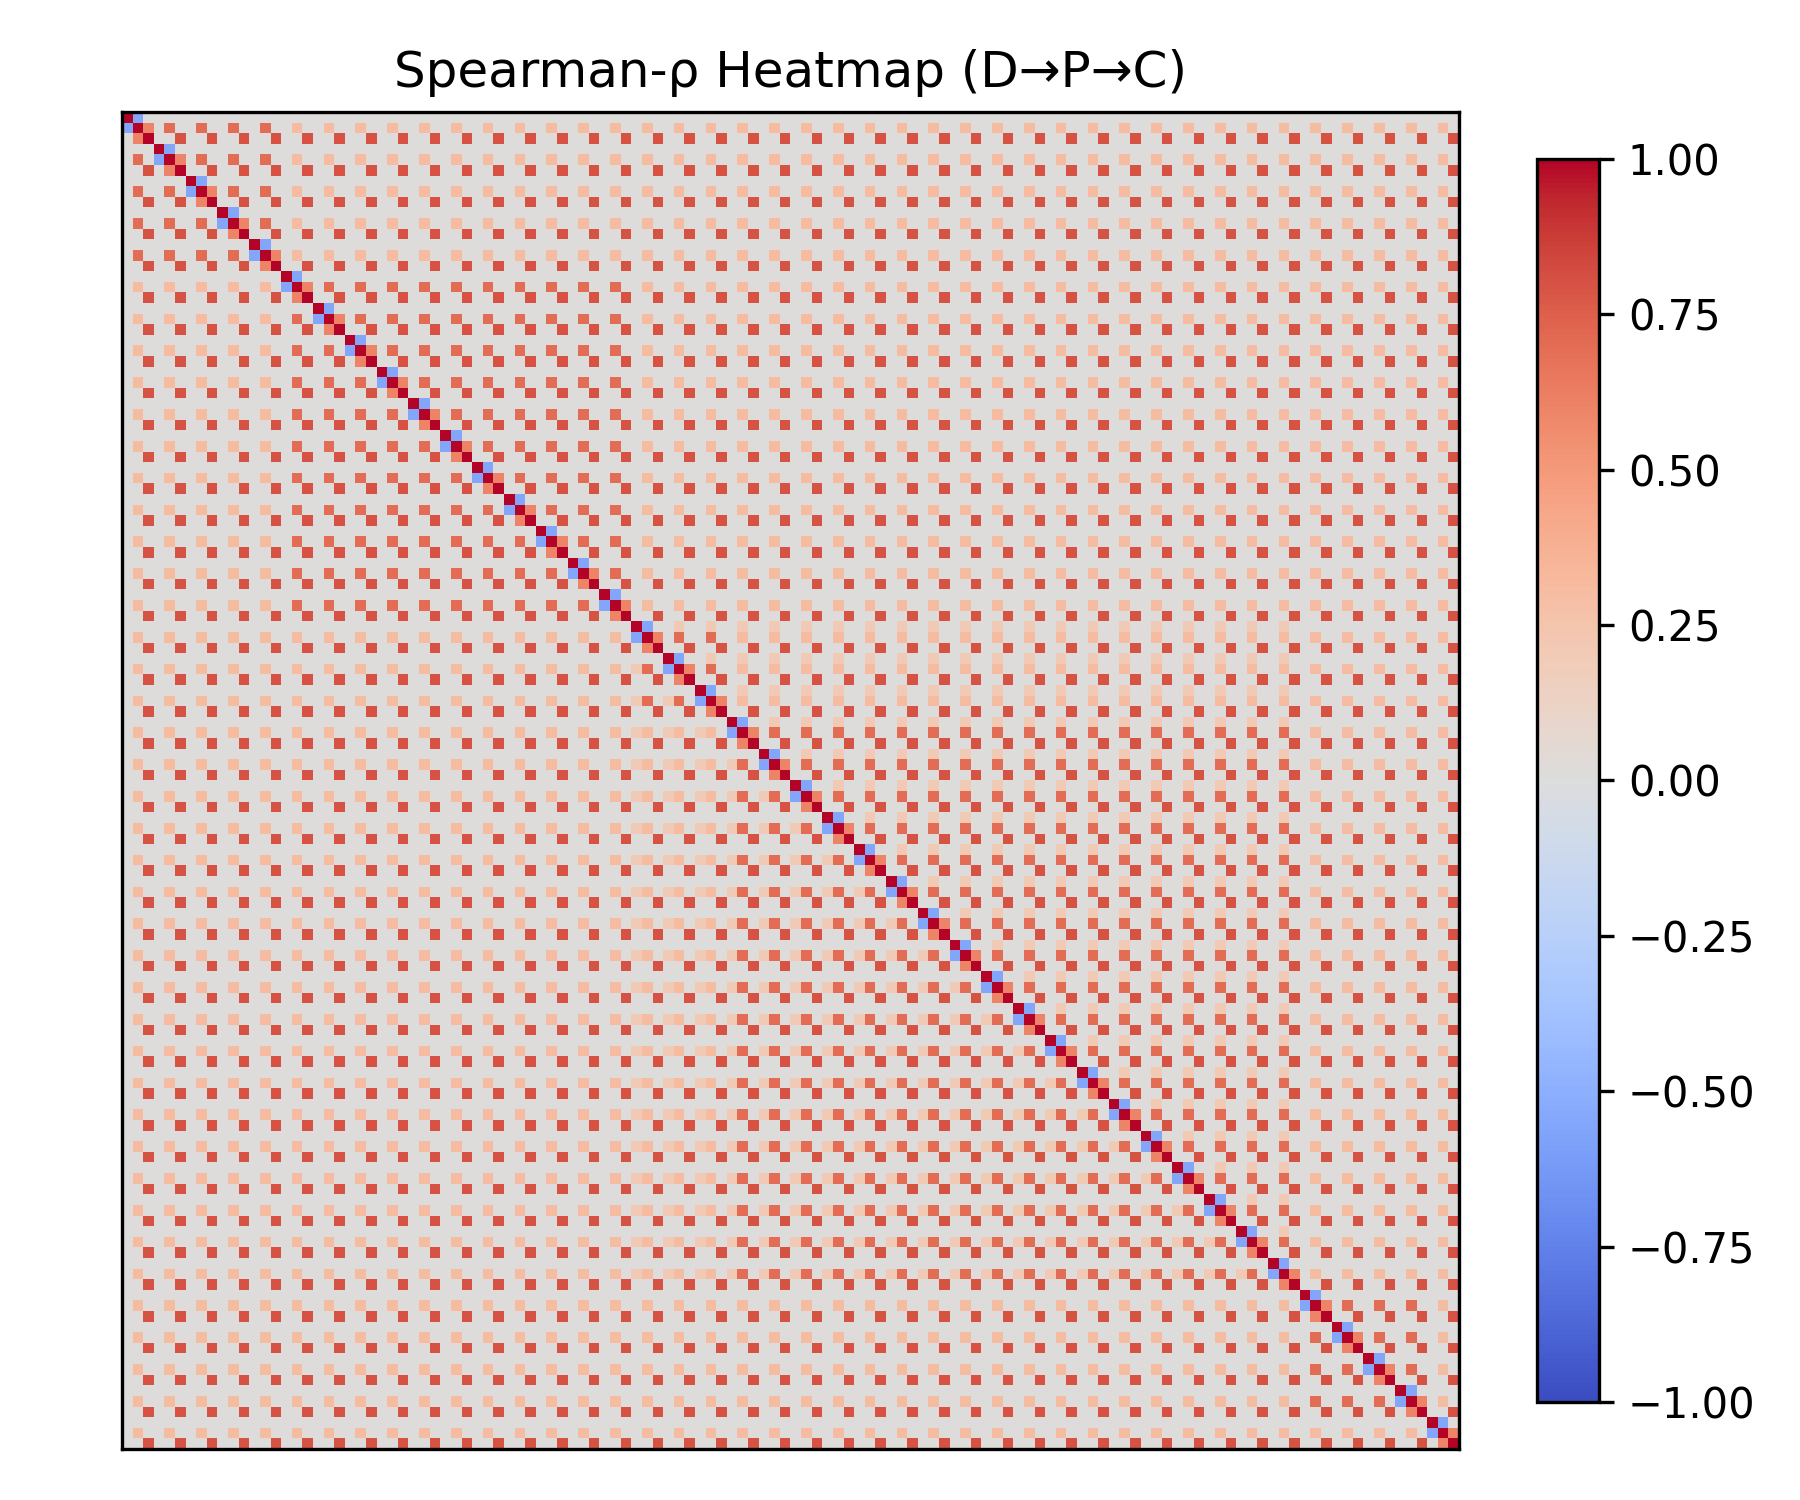
\includegraphics[width=0.86\linewidth]{figures_pb3/d6b01d20396794b667c82f8a2af2b5b5.png}
  \caption{Spearman-$\rho$ 相关热力图（$D\!\to\!P\!\to\!C$ 展开顺序）}
\end{figure}

\paragraph{块结构的可解释性} 图~1 展示了 Copula 场景样本的秩相关（Spearman-$\rho$）热力图，沿主对角的 $3\times3$ 作物子块呈现出预期的“$D$-$P$ 负相关、$P$-$C$ 正相关”模式；跨作物之间，同类型价格/成本的相关度更高，符合“同类市场共振”的直觉。:contentReference[oaicite:2]{index=2}

\begin{figure}[htbp]
  \centering
  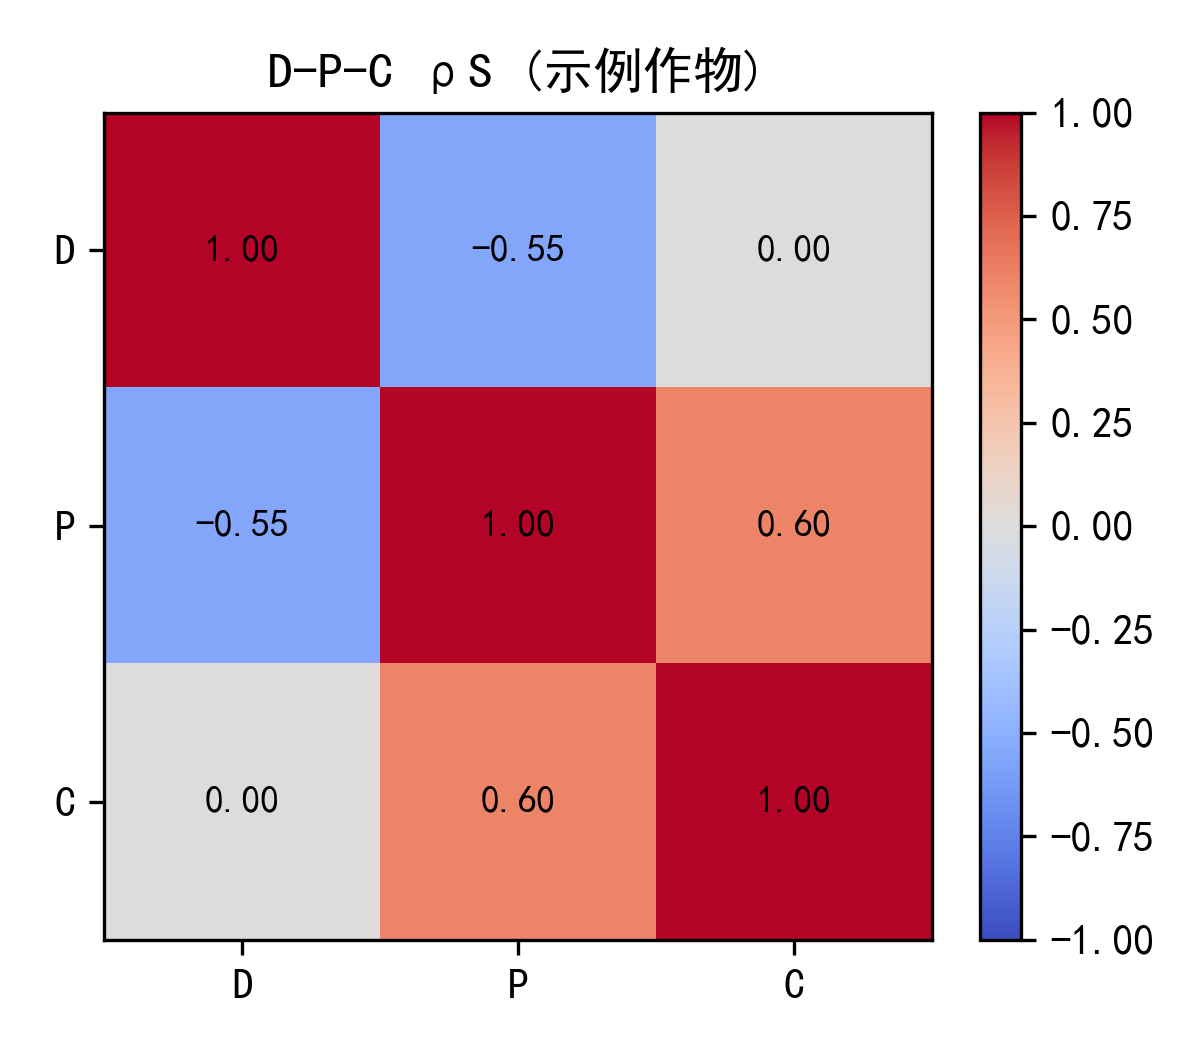
\includegraphics[width=0.7\linewidth]{figures_pb3/triple_block.png}
  \caption{单作物 $D$-$P$-$C$ 的秩相关检验（示例作物）}
\end{figure}

\paragraph{Copula 样本的秩散点检验} 进一步对“价格秩—需求秩”进行散点检验（图~3、图~6），可见整体呈“右上稀、左上密”的斜负型云图，印证 $P\uparrow$ 时 $D\downarrow$ 的负相关设定；点云并非线性，说明 Copula 允许\emph{非线性}相关形态并保留重尾的可能。:contentReference[oaicite:3]{index=3}

\begin{figure}[htbp]
  \centering
  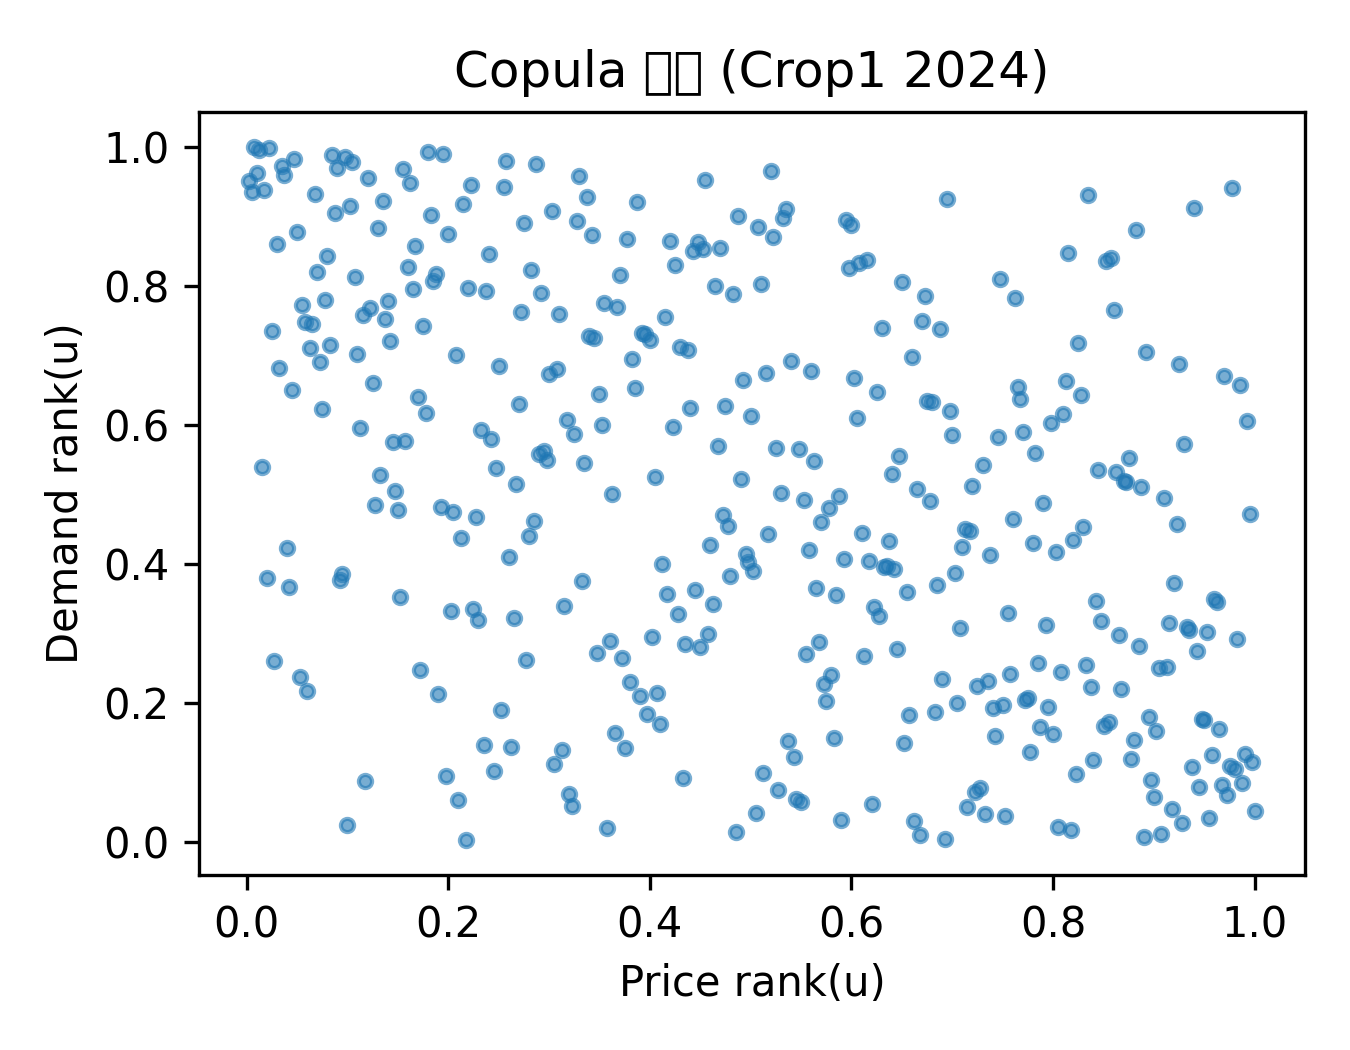
\includegraphics[width=0.78\linewidth]{figures_pb3/0548217d8d83c8fb195137e3cf3cc2b5.png}
  \caption{Copula 检验：价格秩 vs 需求秩（Crop1, 2024）}
\end{figure}

\begin{figure}[htbp]
  \centering
  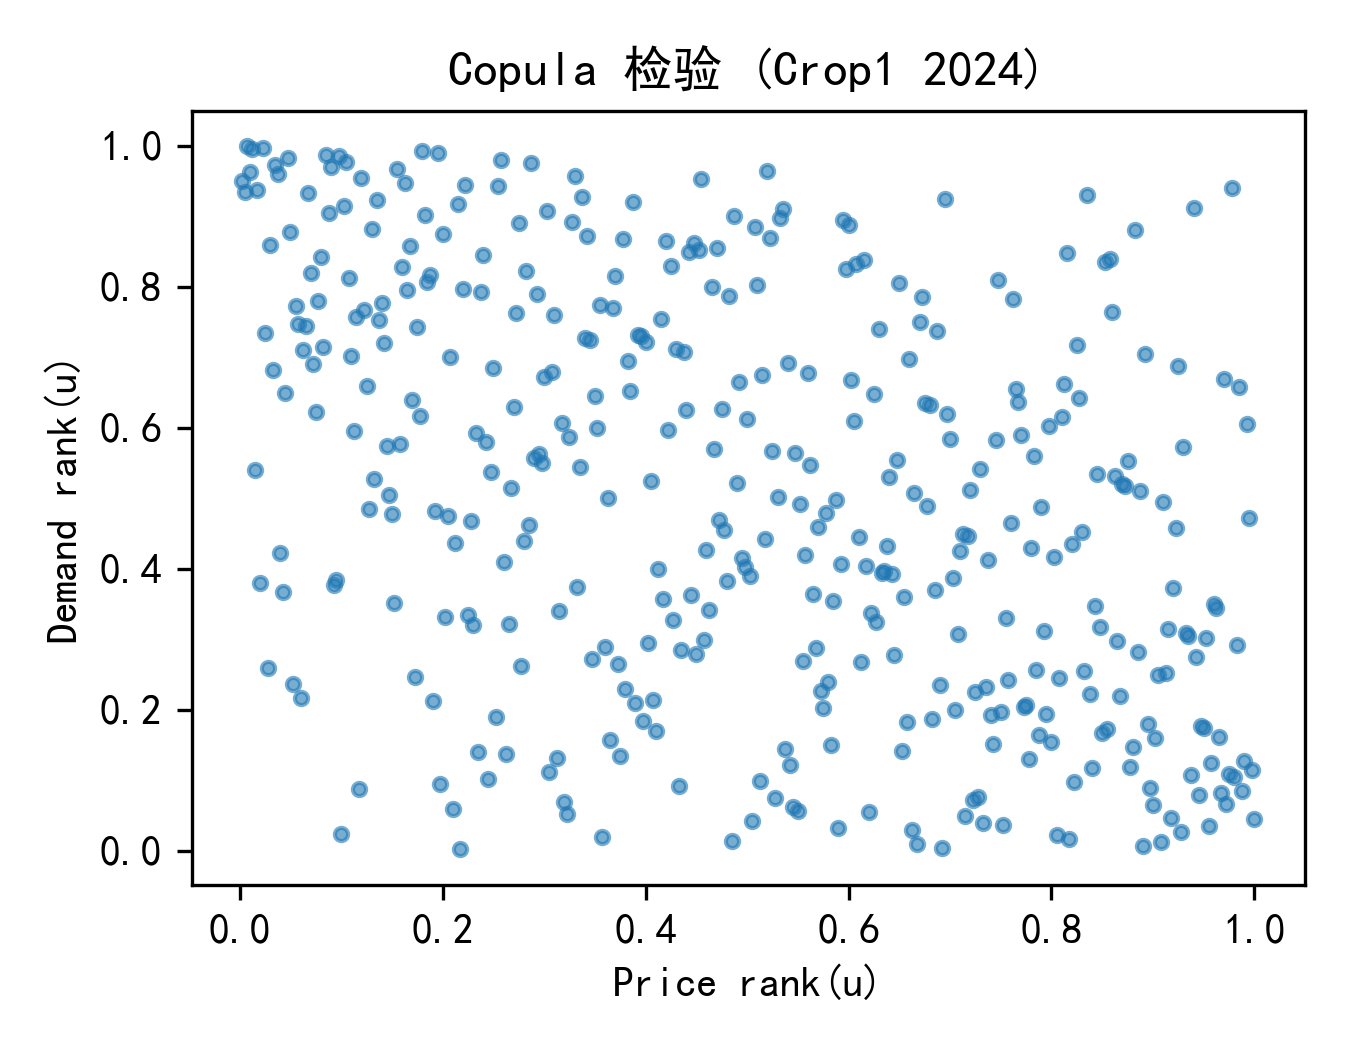
\includegraphics[width=0.78\linewidth]{figures_pb3/copula_rank_scatter.png}
  \caption{Copula 检验（另一可视化样式）：价格秩 vs 需求秩}
\end{figure}

\subsection{含相关性与替代/互补的情景优化模型}
\paragraph{需求的交叉弹性修正} 在 Copula 生成的 $(D,P,C)$ 基础上，用
\[
D_i^{\text{adj}} \;=\; D_i \Big(1+\sum_{j} \varepsilon_{ij}\,\Delta p_j\Big),\qquad 
\Delta p_j=\frac{P_j-P_j^{(0)}}{P_j^{(0)}}
\]
对需求进行一次线性修正：蔬菜—蔬菜设置弱替代 $(\varepsilon_{ij}\!>\!0)$，部分“粮食—豆类”设互补 $(\varepsilon_{ij}\!<\!0)$，从而把“\emph{作物间的相对价格变化会改变各自销量上限}”这一经济逻辑显式注入情景。:contentReference[oaicite:4]{index=4}

\paragraph{目标函数与约束} 目标仍为
\[
\max\ \ \mathbb{E}[\Pi]-\lambda\cdot \mathrm{CVaR}_{0.95}(\text{亏损}),
\]
收益按“需求内原价、超出部分 $50\%$ 折价”计；农艺与管理约束（适宜性、禁重茬、三年豆类覆盖、分散度）与问题二一致，并以大罚分融入适应度。GA 采用整数编码、两点交叉、均匀变异与锦标赛选择。:contentReference[oaicite:5]{index=5}

\subsection{结果：风险—收益权衡与对比}
\paragraph{风险—收益前沿} 通过调节 $\lambda\!\in\!\{0,\ 0.05,\ 0.10,\ 0.15,\ 0.20\}$ 得到的最优解构成“期望利润—CVaR95\%（亏损）”的前沿（图~5）。随着 $\lambda$ 提高（越保守），CVaR 显著下降而期望利润有所回落，呈现典型的\emph{凹型权衡}；这说明在存在相关冲击与替代/互补时，增加风险厌恶可有效削减尾部亏损。:contentReference[oaicite:6]{index=6}

\begin{figure}[htbp]
  \centering
  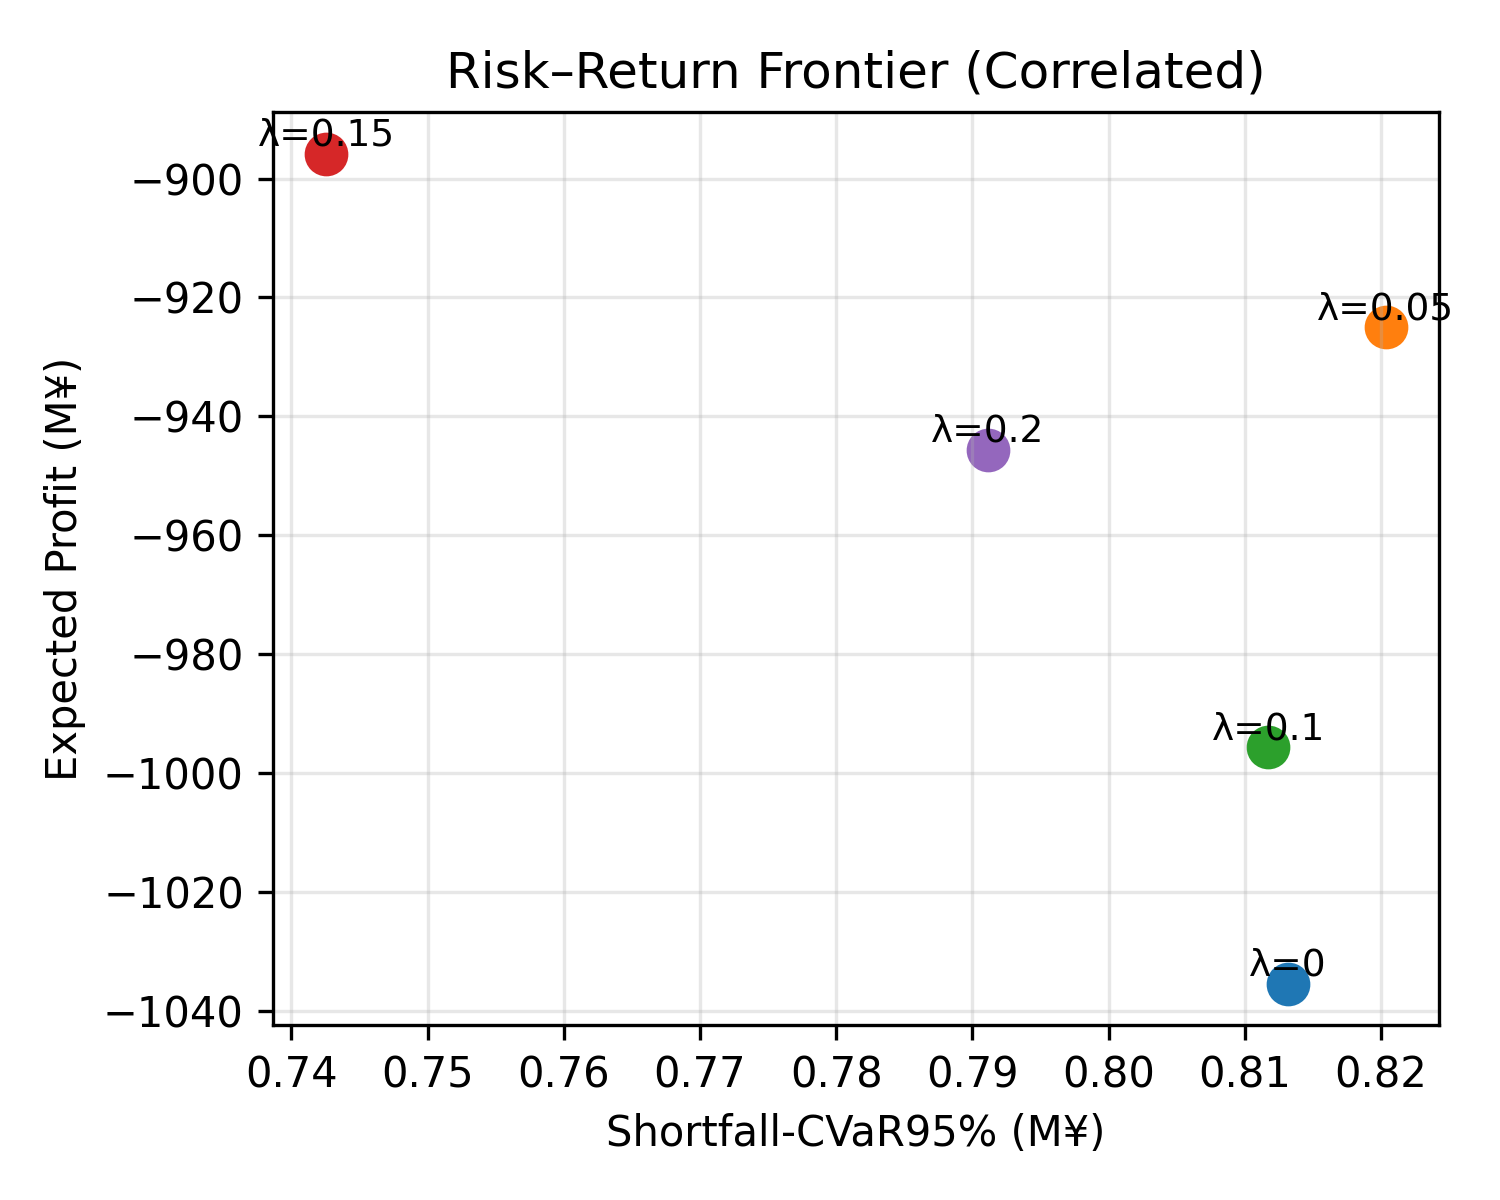
\includegraphics[width=0.82\linewidth]{figures_pb3/34f1e36d36fcf15b8c48d02c32728306.png}
  \caption{含相关性的风险—收益前沿（不同 $\lambda$）}
\end{figure}

\paragraph{与问题二的差异点（定性）}
\begin{itemize}
  \item \textbf{相关冲击：} 价格与成本共振、同类作物价格联动，使得单一作物“加仓”带来的边际收益递减更快；  
  \item \textbf{结构调整：} 弹性项促使需求在替代组间再分配，最优解出现\emph{更强的多样化}与\emph{跨组错峰}；  
  \item \textbf{风险收敛：} 在相同迭代规模下，GA 的最优值提升幅度较问题二更平缓，但尾部风险（CVaR）下降更显著，体现了“相关风险管理”的价值。  
\end{itemize}

\subsection{管理启示}
\begin{enumerate}
  \item \textbf{价格—销量联动要纳入长周期配置：} 当同类作物价格一并走弱时，替代效应无法完全对冲，需要通过\emph{跨类型}与\emph{跨季}的多样化来稳收益；  
  \item \textbf{设置风控档位：} 以 $\lambda$ 为旋钮可生成一条\emph{面向管理者风险偏好}的可选方案带；  
  \item \textbf{弹性参数的校准：} 可用历史价格—销量数据或专家打分来校准 $\varepsilon_{ij}$，并定期滚动更新，以避免结构性偏差。  
\end{enumerate}

\begin{figure}[htbp]
  \centering
  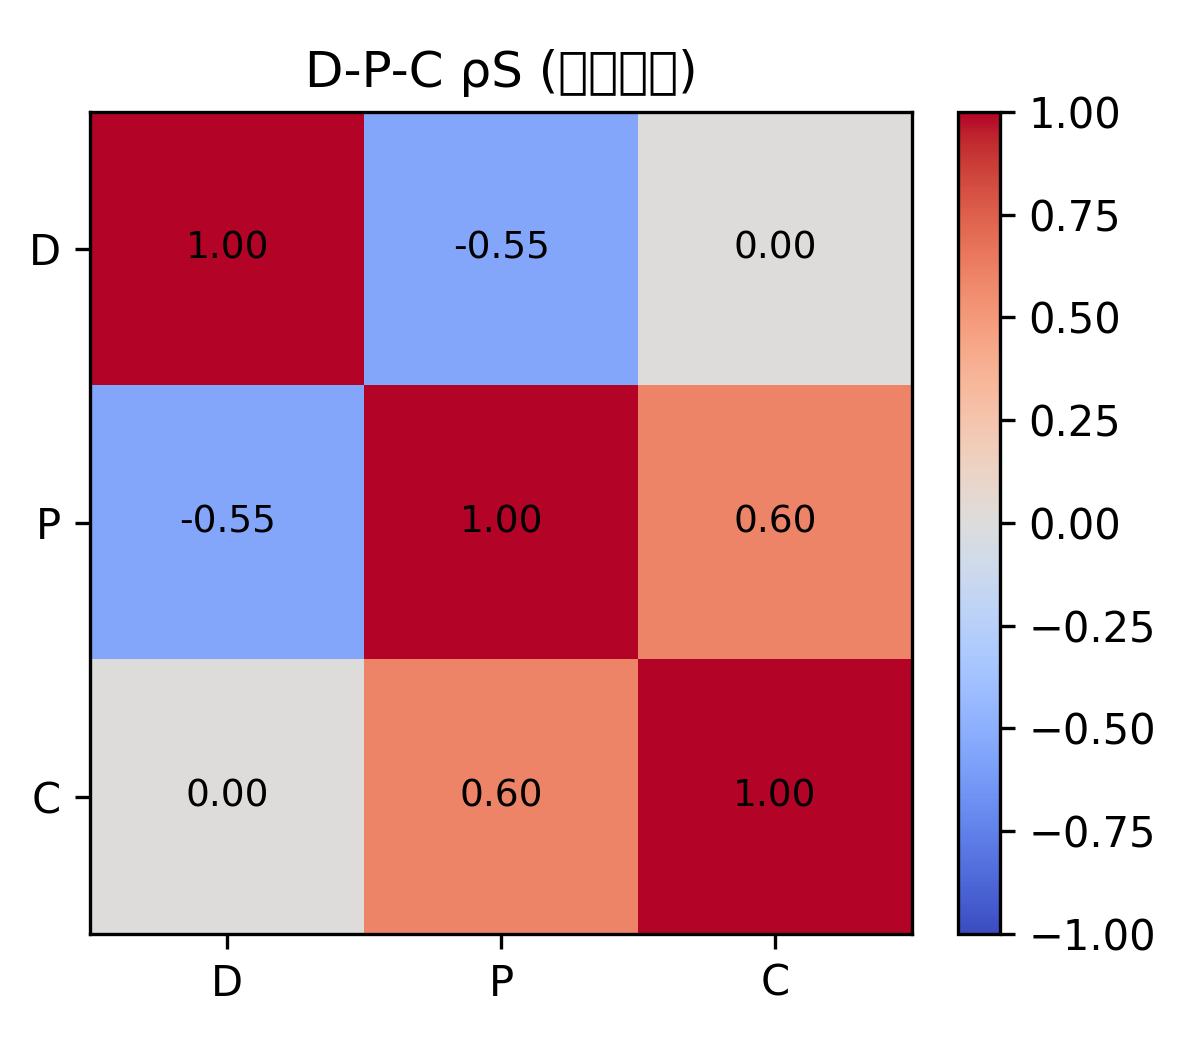
\includegraphics[width=0.72\linewidth]{figures_pb3/b40bf6b78dcf876c31f5a06c33aea3a6.png}
  \caption{单作物 $D$-$P$-$C$ 的秩相关检验（中文标注版本）}
\end{figure}

\noindent\textbf{小结：} 问题三通过 Copula 与交叉弹性，将\emph{作物间可替代/互补}与\emph{价格—成本—销量相关}纳入多年期排作优化；在相同的农艺与管理约束下，所得方案在风险调整口径（CVaR）上显著优于不考虑相关性的情景，同时保留了较高的期望收益。模型、算法与可视化流程详见 \verb|problem3.py|。:contentReference[oaicite:7]{index=7}
